\documentclass[11pt]{beamer}
\mode<presentation>
\let\Tiny=\tiny
\usetheme{CambridgeUS}
\usefonttheme{professionalfonts}
\usepackage[brazil]{babel}
\usepackage[utf8]{inputenc}
\usepackage{amsfonts}
\usepackage{amssymb}
\usepackage{amsmath}
\newtheorem{mydef}{Definição}
\newtheorem{myexample}{Exemplo}

\title{Introdução à \textit{internet}}
\author{}
\date{}

\begin{document}

    \begin{frame}[plain]
        \titlepage
    \end{frame}

    \section{Introdução}

    \begin{frame}{Introdução}
      \begin{itemize}
        \item Entender como funciona a \textit{internet} é importante para o desenvolvimento de aplicações \textit{web}.
        \item Apesar de muitas ferramentas automatizarem tarefas, a correta compreensão de como a informação trafega na \textit{internet} pode auxiliar a resolver problemas que necessitam de algum ajuste fino.
      \end{itemize}
    \end{frame}

    \begin{frame}{Introdução}
      \begin{itemize}
        \item A \textit{internet} é simplesmente a intercomunicação de diferentes redes de computadores.
        \item As diversas redes comunicam-se através de grandes roteadores que ligam o planeta quase todo.
      \end{itemize}
    \end{frame}

    \begin{frame}{Introdução}
      \begin{itemize}
        \item Como todo sistema computacional, é comum o foco apenas na abstração e o completo esquecimento de que a \textit{internet} funciona sobre uma base física.
        \item Os dados nada mais são que sinais que trafegam em fios.
        \item Dada esta natureza física, é importante ter sempre em mente as limitações dos materiais.
      \end{itemize}
    \end{frame}

    \section{Infraestrutura da \textit{internet}}

    \begin{frame}{Infraestrutura da \textit{internet}}
      \begin{itemize}
        \item A \textit{internet}, assim como as demais redes de computadores, estão organizadas de maneira hierárquica.
        \item Há grandes NSP (\textit{Network Service Providers}) interligados por NAPs (\textit{Network Access Points}).
        \item Os NSPs também estão ligados a ISPs regionais que, por sua vez, estão ligados a ISPs locais. 
        \item Os dispositivos de pessoas comuns e empresas estão ligados aos ISPs locais.
        \item A informação que sai de um computador vai a um ISP local, passa a um ISP regional, depois a NSP e, se necessário ainda, pode ir a outro NSP através de um NAP.
      \end{itemize}
    \end{frame}

    \begin{frame}{Infraestrutura da \textit{internet}}
      \begin{figure}
        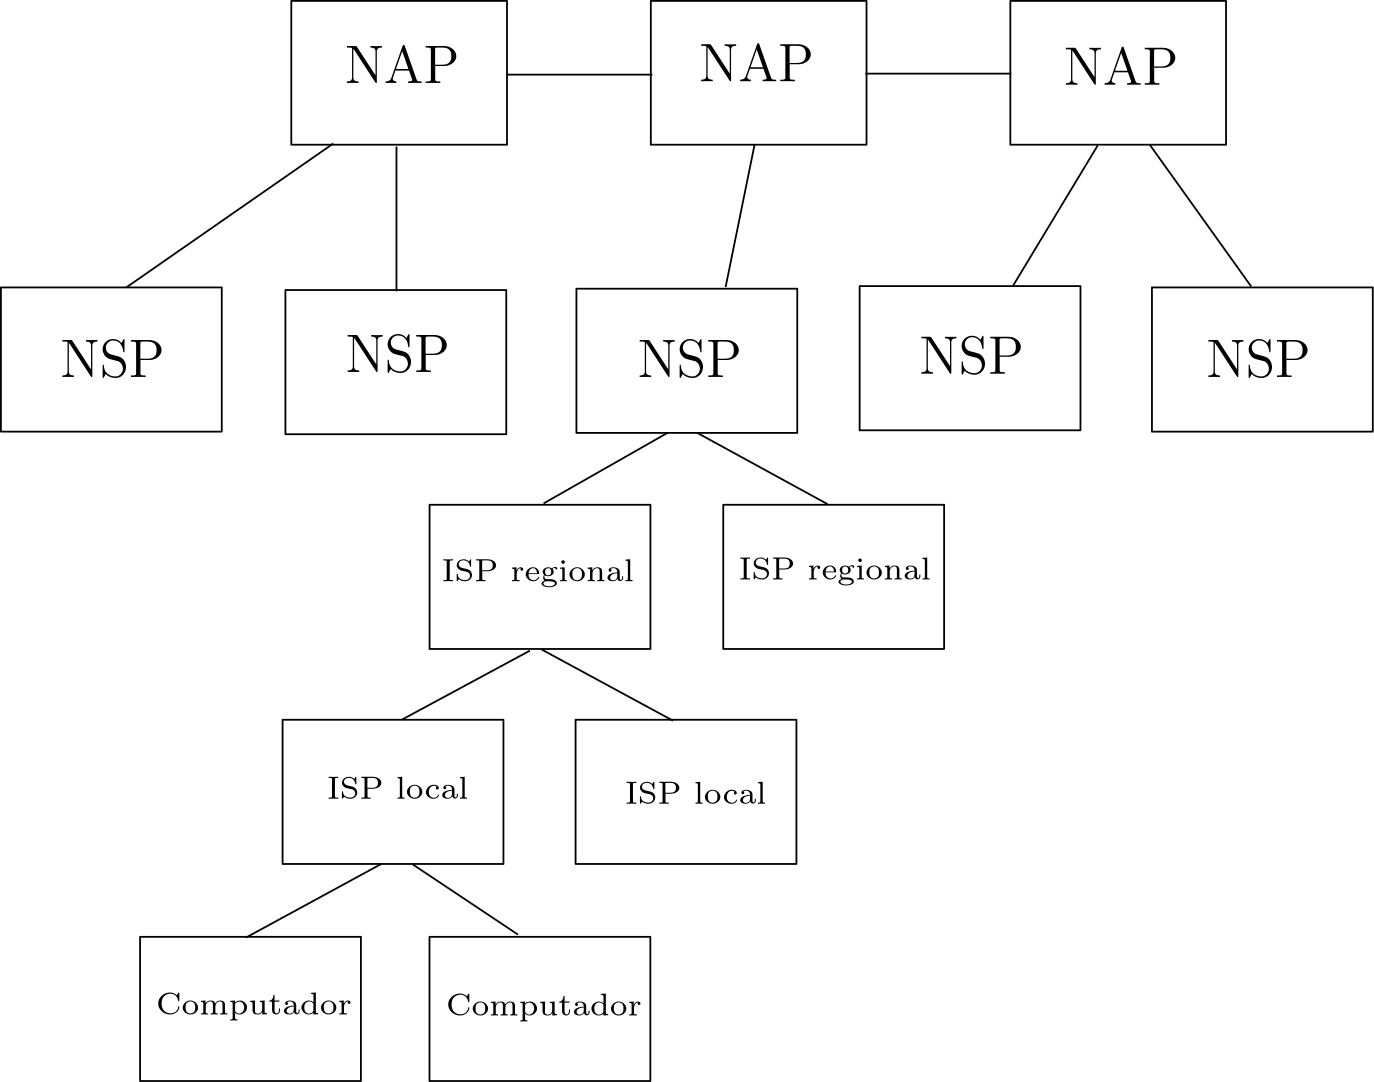
\includegraphics[width=8cm, height=6cm]{figures/hierarquia_internet.png}
      \end{figure}
    \end{frame}

    \begin{frame}{Infraestrutura da \textit{internet}}
      \begin{itemize}
        \item Como é impossível que todos os dispositivos saibam onde estão localizados todos os demais dispositivos conectados à internet, a ligação entre os diferentes \textit{backbones}\footnote{Redes de comunicação de alta velocidade.} dos provedores é realizada através de roteadores.
        \item Cada roteador possui uma tabela de roteamento que permite escolher o melhor caminho para enviar um pacote de informação.
        \item Os dados trafegam por linhas físicas e que podem estar congestionadas. Então, o roteador deve escolher o caminho mais rápido.
      \end{itemize}
    \end{frame}

    \section{Protocolos}
    
    \begin{frame}{Protocolos}
      \begin{itemize}
        \item Dada a quantidade de diferentes dispositivos e tipos de redes de computadores, foi necessário estabelecer protocolos de comunicação.
        \item Um protocolo de comunicação é uma série de regras que estabelece parâmetros e fluxos de comunicação.
        \item Através de um protocolo é possível a comunicação entre redes e dispositivos dos mais diversos fabricantes. 
      \end{itemize}
    \end{frame}

    \begin{frame}{Protocolos}
      \begin{itemize}
        \item Um protocolo único, porém, não é desejado, já que é difícil estabelecer uma regra universal.
        \item Apesar da \textit{internet} como rede estar bem padronizada, as aplicações que rodam sobre esta infraestrutura evoluem rapidamente e necessitam de protocolos sempre mais atualizados que sejam condizentes com suas necessidades. 
      \end{itemize}
    \end{frame}

    \begin{frame}{Protocolos}
      \begin{itemize}
        \item A \textit{internet} e suas aplicações funcionam com uma pilha de protocolos.
        \item Cada protocolo age em um determinado aspecto.
        \item Os aqui chamados aspectos são técnicamente chamados de camadas.
        \item Cada camada tem suas responsabilidades e protocolos.
        \item Há protocolos para gerir o funcionamento das aplicações, do transporte de informações e da organização da rede.
      \end{itemize}
    \end{frame}

    \subsection{Camada de internet}

    \begin{frame}{\textit{Internet Protocol} (IP)}
      \begin{itemize}
        \item O protocolo que organiza os dispositivos na \textit{internet} (camada de internet) é o \textit{Internet Protocol} (IP).
        \item Ao conectar-se à internet através de um ISP, o dispositivo recebe um endereço IP temporário.
        \item Os servidores possuem endereços fixos. 
        \item O endereço IP é formado por uma sequência numérica que tem formato variado de acordo com a versão do IP adotada.
      \end{itemize}
    \end{frame}

    \subsection{DNS}

    \begin{frame}{\textit{Domain Name Service} (DNS)}
      \begin{itemize}
        \item Como os endereços IP são sequências numéricas de difícil memorização por seres humanos, criaram-se domínios.
        \item Os domínios são pseudônimos que permitem que os usuários possam digitar palavras ao invés de ter de decorar os endereços IPs.
        \item Exemplos de domínio são google.com, yahoo.com, etc.
      \end{itemize}
    \end{frame}

    \begin{frame}{\textit{Domain Name Service} (DNS)}
      \begin{itemize}
        \item Após o usuário solicitar um endereço de domínio no navegador, o navegador busca o endereço IP deste domínio através do \textit{Domain Name Service} (DNS).
        \item O DNS é composto por uma série de servidores com tabelas indicando o endereço IP de cada domínio.
        \item Assim que recupera o endereço IP do domínio desejado, o navegador prossegue na tentativa de estabelecer conexão com o servidor localizado no dado endereço.
      \end{itemize}
    \end{frame}

    \subsection{Camada de transporte}

    \begin{frame}{\textit{Transmission Control Protocol} (TCP)}
      \begin{itemize}
        \item O estabelecimento da conexão entre clientes e servidores é feito na camada de transporte.
        \item O protocolo da camada de transporte mais comum é o \textit{Transmission Control Protocol} (TCP).
        \item Junto com o IP, o TCP é responsável por uma grande fatia de tráfego na \textit{internet}.  
      \end{itemize}
    \end{frame}

    \begin{frame}{\textit{Transmission Control Protocol} (TCP)}
      \begin{itemize}
        \item O TCP é responsável por encapsular a mensagem em pacotes que serão transmitidos pacotes, além de estabelecer as regras da conexão entre os dispositivos.
        \item O TCP é considerado confiável, pois ele estabelece que todos os pacotes devem ser entregues.
        \item Em caso de perda, o pacote será reenviado.
        \item A confiabilidade torna, porém, a comunicação mais lenta, pois assim que o pacote é recebido, deve-se enviar uma mensagem confirmando seu recebimento.
        \item 
      \end{itemize}
    \end{frame}

    \begin{frame}{\textit{User Datagram Protocol} (UDP)}
      \begin{itemize}
        \item No caso de aplicações em que a perda de dados é tolerada, tem-se o UDP (\textit{User Datagram Protocol}).
        \item No UDP, não há confirmação de recebimento e, por conseguinte, reenvio de pacotes perdidos.
        \item Este protocolo é menos confiável, mas muito mais rápido, sendo o ideal para aplicações em tempo real em que a perda de pacotes não seja sentida, como jogos, transmissões ao vivo, etc.
      \end{itemize}
    \end{frame}

    \begin{frame}{Camada de transporte}
      \begin{itemize}
        \item Se a informação a ser enviada for muito grande, o protocolo de transporte (TCP ou UDP) pode quebrar a informação em diversos pacotes numerados e organizados em uma fila.
        \item Os pacotes são endereçados a uma porta específica do dispositivo recebedor. As aplicações no dispositivo recebedor devem "ouvir" a uma porta específica.
      \end{itemize}
    \end{frame}

    \subsection{Camada de aplicação}

    \begin{frame}{Camada de aplicação}
      \begin{itemize}
        \item As camadas de transporte e redes não são o suficiente para rodar as aplicações na \textit{internet}.
        \item Elas definem apenas a organização da rede e o modo de comunicação entre dois dispositivos.
        \item A maneira como as aplicações sobre esta estrutura irão funcionar é definida pelos protocolos de aplicação.
        \item O protocolo de aplicação varia de acordo com o tipo de aplicação (hipertexto, e-mail, transferência de arquivos, etc.)
      \end{itemize}
    \end{frame}

    \begin{frame}{\textit{Hypertext Transfer Protocol} (HTTP)}
      \begin{itemize}
        \item Para utilizar a *World Wide Web* (WWW), o protocolo utilizado é o *Hypertext Transfer Protocol* (HTTP).
        \item Ele define como as mensagens em hipertexto serão transferidas entre os dispositivos.
      \end{itemize}
    \end{frame}

    \begin{frame}{\textit{Hypertext Transfer Protocol} (HTTP)}
      \begin{itemize}
        \item No HTTP há duas entidades, clientes e servidores.
        \item Toda conexão HTTP deve ser iniciada pelo cliente, apesar de que, com o passar do tempo, tenham sido criados mecanismos que simulam mensagens iniciadas pelo servidor).
        \item O servidor recebe essa requisição e envia uma resposta.
        \item Por exemplo, quando é digitado um endereço em um navegador \textit{web}, o que se está fazendo é uma requisição a um servidor.
        \item O servidor processa essa requisição e devolve um hipertexto a ser exibido no navegador cliente.
      \end{itemize}
    \end{frame}

    \begin{frame}{\textit{Hypertext Transfer Protocol} (HTTP)}
      \begin{itemize}
        \item O HTTP não controla o transporte dos pacotes, mas exige que as mensagens sejam enviadas através de um protocolo confiável, como o TCP. Antes de iniciar uma conexão HTTP, é necessário estabelecer uma conexão TCP.
        \item Para o HTTP, cada requisição é uma conexão independente de suas anteriores (\textit{stateless}).
        \item O uso de \textit{cookies} permite \textit{stateful sessions}.
      \end{itemize}
    \end{frame}

    \begin{frame}{\textit{Hypertext Transfer Protocol} (HTTP)}
      A requisição HTTP tem como elementos principais:
      \begin{itemize}
        \item método;
        \item endereço IP e porta;
        \item versão do protocolo;
        \item outros dados opcionais.
      \end{itemize}
    \end{frame}

    \begin{frame}{\textit{Hypertext Transfer Protocol} (HTTP)}
      Os principais métodos HTTP são:
      \begin{itemize}
        \item GET $\rightarrow$ para requisições simples;
        \item POST $\rightarrow$ para enviar valores ao servidor;
        \item PUT $\rightarrow$ similiar ao POST, porém idempotente;
        \item DELETE $\rightarrow$ para excluir recursos.
      \end{itemize}
    \end{frame}

    \begin{frame}{\textit{Hypertext Transfer Protocol} (HTTP)}
      A resposta HTTP tem como elementos principais:
      \begin{itemize}
        \item versão do protocolo;
        \item código de \textit{status};
        \item mensagem de \textit{status};
        \item cabeçalhos;
        \item resposta.
      \end{itemize}
    \end{frame}

    \section{Conclusão}

    \begin{frame}{Fluxo da \textit{internet}}
      Em resumo, a \textit{internet} tem o seguinte fluxo básico:
      \begin{itemize}
        \item o usuário digita a URL (\textit{Uniform Resource Location}) no seu navegador;
        \item o navegador faz uma consulta ao DNS pelo endereço IP correspondente à URL, se ele não o tiver;
        \item é iniciada uma conexão TCP através de um aperto de mão de três vias, onde são negociados parâmetros da conexão TCP;
        \item negociação de TLS, onde cliente e servidor negociam qual será o padrão de criptografia de dados;
        \item navegador realiza a requisição HTTP;
        \item servidor responde a requisição;
      \end{itemize}
    \end{frame}

    \begin{frame}{Referências}
      \begin{itemize}
        \item Akhmed, Kamran. How does the internet work? https://roadmap.sh/guides/what-is-internet
        \item Shuler, Rus. How does the internet work? 2002 https://web.stanford.edu/class/msande91si/www-spr04/readings/week1/InternetWhitepaper.htm (necessita atualização)
        \item Mestrado em Redes e Serviços de Comunicação - Faculdade de Engenharia da Universidade do Porto. https://paginas.fe.up.pt/~mrs01003/TCP\_IP.htm
        \item CloudFlare. What is in an HTTP request? https://www.cloudflare.com/en-gb/learning/ddos/glossary/hypertext-transfer-protocol-http/
        \item Mozilla Developer Network. An overview of HTTP. 2023. https://developer.mozilla.org/en-US/docs/Web/HTTP/Overview
      \end{itemize}
    \end{frame}

    \begin{frame}{Referências}
      \begin{itemize}
        \item Garsiel, Tali e Irish, Paul. How browsers work. 2011. https://web.dev/howbrowserswork/
        \item Mozilla Developer Network. Populating the page: how browsers work. 2023. https://developer.mozilla.org/en-US/docs/Web/Performance/How\_browsers\_work
      \end{itemize}
    \end{frame}

\end{document}